%\documentclass[a4paper, twocolumn]{article}
\documentclass[a4paper]{article}
\newcommand{\papertitle}{Whitepaper}

\usepackage[a4paper, margin=2cm]{geometry}

\usepackage[utf8]{inputenc}
\usepackage[T1]{fontenc}
\usepackage{graphicx}
\usepackage[english]{babel}
\usepackage[colorlinks=true,urlcolor=red]{hyperref}
\usepackage{url}
\usepackage{float}
\usepackage{cleveref}
\usepackage{todonotes}

\usepackage{multicol}
\setlength{\columnsep}{1cm}

\usepackage{fancyhdr}
\fancyhead{}
\fancyfoot{}
\fancyhead[l]{\papertitle}
\fancyhead[r]{\includegraphics[height=1em]{esiwacelogo_type_grey_left_2c_ext}}
\fancyfoot[r]{\thepage}
\pagestyle{fancy}
\renewcommand{\headrulewidth}{1pt}
\renewcommand{\footrulewidth}{1pt}

\usepackage{titling}
\pretitle{\begin{center}\Large\bfseries}
\posttitle{\end{center}\vskip 0.5em}

\graphicspath{{./assets/}}

\title{\papertitle}

\author{Julian M. Kunkel
  \textit{University of Reading}
	\and
  Luciana R. Pedro
  \textit{University of Reading}
}
\date{\today}


\begin{document}
\maketitle
\thispagestyle{fancy}

\section*{Abstract}

\section{Introduction}

\section{Workflows}
\label{sec:background}

An example of a simple workflow can be seen in \Cref{fig:workflow}. In this workflow, there are the following components:

\begin{description}

\item[Input] The data inserted in the workflow. It is composed of files describing, for instance:

\begin{itemize}

\item The actual input data, for instance, the dates for the experiments, how many times the workflow has to run,

\item The dependencies among the tasks. In this case, Task 1 and Task 3 have no dependencies and Task 2 depends on the results of Task 1.

\item The I/O information, i.e., where the data will be storage in each step of the workflow.

\item The information about how long the final result has to be stored.

\item The steps in which manual decisions have to be made.

\end{itemize}

For simplicity, we will call these files as \texttt{input-workflow.conf}.

\item[Task 1] The task is specified by the user and the information we have about it are:

\begin{itemize}

\item The data input.

\item The data output.

\item How long the data has to be stored.

\item The dependencies regarding the other tasks.

\end{itemize}

In case of Task 1, we have:

\begin{itemize}

\item Task 1 has no prior dependencies other than the general input.

\item Task 1 is a dependency for running Task 2.

\item For simplification purposes, we will assume that Task 1 has the files \texttt{input1.conf}, \texttt{output1.conf}, and \texttt{storage1.conf} as descriptors.

\end{itemize}

\item[Task 2]

\begin{itemize}

\item Task 2 is a dependent of Task 1.

\item Task 2 has the files \texttt{input2.conf}, \texttt{output2.conf}, and \texttt{storage2.conf} as descriptors.

\end{itemize}

\item[Task 3]

\begin{itemize}

\item Task 3 is independent. It does not require any other task to be started and, after finished, no other task will use its results other than the general output.

\item Task 3 has the files \texttt{input3.conf}, \texttt{output3.conf}, and \texttt{storage3.conf} as descriptors.

\end{itemize}

\item[Output]

The output consists of all files generated by the workflow. Those files have to be stored for a specific amount of time previously described in one of the input files.

For simplicity, we will call these files as \texttt{output-workflow.conf}. In this specific example, it is composed by the files \texttt{output1.conf}, \texttt{output2.conf}, and \texttt{output3.conf}.

\end{description}

\begin{figure}[b]
  \centering
%  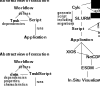
\includegraphics[width=0.75\columnwidth]{workflow}
  \caption{Example High-Level Workflow}
  \label{fig:workflow}
\end{figure}

For the purposes of this work, the files belonging to \texttt{input-workflow.conf} are the files inserted as input for the running Cylc. The Cylc tool receives, as predefined, information about the storage and dependencies of the files. These information are used to contructed and run the complete workflow, but it is not used to optimise intermediate steps. Some things are already predefined and they cannot change. For instante, if it is estabilished that Task 2 depends on Task 1, then we have to wait for Task 1 to be completed to start running Task 3. But several things can be optimised if we know the whole workflow in advance. For instance: Task 1 and Task 3 have no previous dependencies. How do we decide about when we should run those tasks? Task 1 first, because it is a dependency for Task 2? Task 3 first, because then we have a previous of a complete result, considering Task 3 has no dependencies at all? Can Task 1 and Task 3 run in parallel at the same time, and then the workflow only has to complete Task 2 to finish? On the contrary, Task 1 is really processing demanding, so it should run alone and then Task 2 and Task 3 can run concurrently without extra burden to the computing time? These are all concerns about processing time and the dependencies. But what about I/O? No decision is being made about an optimal way to store the data. Consider, for instance, that the files from \texttt{output1.conf} are divided into \texttt{output1-final.conf} and \texttt{output1-task2.conf}. Then, it is clear that \texttt{output1-task2.conf} will be required to run Task 2, and because of that, should be put in a fast storage to quickly being retrieved, of even kept in local storage. The \texttt{output1-final.conf} files, however, can go directly to tape, if the lifetime of the final output has to be stored for five years.

Those simple examples are here to demonstrate that, once we have the complete knowledge about how the workflow is expect to run, we can optimise steps that were before predefined by the user considering only the options for feasibility. The user input is one of the viable options to run the workflow, but probably it is not the best, assuming other options are available. The user might even have analysed other options, but s/he has done that in a naive way (usually trial and error). By automatising these tasks, specifically a smarter route for the tasks taking into consideration the architecture available and the way the files are stored during the intermediate steps of the workflow, we have a twofold gain:

\begin{itemize}

\item The user does not have to worry about the architecture that the workflow will use, removing from the specialist the decision-making process; and

\item The workflow will be optimised for the specific workflow without extra input from the user and the resources will, then, be better utilised.

\end{itemize}

In this paper, we approach two ways to have the extra information from the user to be able to make decisions about storage and the processing of the files/tasks.

\begin{itemize}

\item The user will insert this information as an extra file to the Cylc workflow management. In fact, the user is already doing that, but he is doing that in just one specific way, to make the workflow possible. Here, we are thinking about simplifying the information the user is already providing. So, instead of giving the complete workflow to Cylc, Here, we are expeting the user to provide really simple information, like:

\begin{description}

\item[Dependencies] Run Task 1 and Task 3 in any specific order and then run Task 2 after Task 1 is finished.

\item[Time/Processing]

\begin{itemize}

\item Task 1 usually requires ten hours running in a pc with standard configuration\footnote{Intel Core i5, 8 GB RAM, and 500 GB internal storage drive, for instance.}, requires 100 GB of storage that has to be persistent for no more than one week.

\item Task 2 usually requires two hours running in a pc with standard configuration, requires 150 GB of storage that has to be persistent for no more than two weeks week.

\item Task 3 usually requires five hours running in a pc with standard configuration and it does not require extra storage other than the storage for the final results.

\end{itemize}

\end{description}

\item The second option to acess this type of information from the user does not require any direct information at all. The idea here is to use the DDN IME Monitoring system and have an estimate for the parameters after one run of the complete workflow. This approach is benefical to the user, because s/he does not have to take any extra step that s/he is currently doing to run the workflow through Cylc, but it the price here is being paid with an extra run of the complete workflow, which can be demanding in both time and price (we are considering here the paid acess to a supercomputer, for example). In the end, it is up to the user and the previous knowledge s/he has about the intermediate stages of the workflow.

\end{itemize}

Now, comes the question. Assuming the information is available, who will be responsible to take the decisions for optimising the storage and the processing tasks? The answer here is simple: the ESDM Scheduler will do it. ESDM Scheduler can be used in different steps of the process. ESDM has already an interface with NetCDF. Assuming the user is able to provide extra information in advance, ESDM can interact in the process before the user provide the data to the Cylc tool, using the information to already contruct an optimised workflow with Cylc) and, once the workflow is constructed by Cylc, ESDM can interact again after the configuration of the scripts for both effective and efficient run of the parallel applications.

This paper intends to describe the information required for the user to run the tools employed in this extended workflow: Cylc (Section ), DDN IME (Section ), and ESDM Scheduler (Section ).

\section{Nice Pictures (or not!)}

Consider the Cylc suite configuration for a toy monthly cycling workflow: a warm-cycled atmospheric model (model) is followed by postprocessing (post), forecast verification (ver), and product generation (prod) tasks \ref{Cylc}. This suite presents the dependencies among the tasks, but it is missing the information about I/O and storage. The decision about where the data with be stored is usually made by the developers in stages prior to Cylc and then it is incorporated into the Cylc process. The decisions about storage have to be made taking into consideration the architecture in which the workflow will run. Applied scientists should not spent time understanding hardware characteristics, but using their time to develop their work, let the computer do the job the simplest way possible, and just collect and analyse the results. However, nowadays, to be able to run a job in a HPC environment, researchers have to have a profound knowledge about their workflow, which is expected, but also about decisions regarding storage, communication, and computing.

We propose an approach to reduce the burden on researchers and, at the same time, optimise the decisions about jobs running in HPC systems. Once we have an automated decision about where the job will run and how the storage will be managed, the scientists can the run their workflows in any machine without further interactions and even without previous knowledge about the machine architecture.

\begin{figure}[H]
  \centering
  \includegraphics[width=0.9\columnwidth]{cylc}
  \caption{Toy Example Workflow}
  \label{fig:cylc}
\end{figure}

Consider one cycle of the workflow, as shown in Figure \ref{fig:cylc-1}. The tasks dependencies are represented by the arrows, but there is no information about the data that are generated. Tasks \texttt{ver} and \texttt{post} depend on Task \texttt{model}, but does Task \texttt{model} needs to be fully completed to satisfy the dependency? Of course once Task \texttt{model} is completed, then Tasks \texttt{ver} and \texttt{post} can proceed, and that is the information Cylc has to create and reproduce the workflow.

\begin{figure}[H]
  \centering
  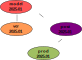
\includegraphics[width=0.4\columnwidth]{cylc-1}
  \caption{First Stage Workflow}
  \label{fig:cylc-1}
\end{figure}

Assume, now, we have the scenario introduced in Figure \ref{fig:cylc-io-model-2}. In this case, we have extra information indicating why Tasks \texttt{ver} and \texttt{post} depend on Task \texttt{model}. In fact, the dependency is not to the complete task, but of some datasets produced by Task \texttt{model}. If this information is available a priori, then we can use it to start Task \texttt{ver} once we have the dataset \texttt{I/O 1} and start Task \texttt{post} once we have the dataset \texttt{I/O 3}, making the general process faster. Still considering this small example, we can assume that dataset \texttt{I/O 2} will not be used for other tasks. So this data can be stored in a "slow" storage or iot can even be deleted.

\begin{figure}[H]
  \centering
  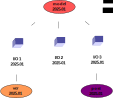
\includegraphics[width=0.6\columnwidth]{cylc-io-model-2}
  \caption{First Stage Workflow}
  \label{fig:cylc-io-model-2}
\end{figure}

Aggregating the information about the datasets produced by every task, we can think about Tasks \texttt{ver}, \texttt{post}, and \texttt{model} as something as depicted in Table \ref{tab:cylc}.

\begin{table}[H]
\centering
\begin{tabular}{|c|c|c|}
\hline
  \includegraphics[width=0.3\columnwidth]{cylc-io-model} &
  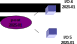
\includegraphics[width=0.3\columnwidth]{cylc-io-post} &
  
\includegraphics[width=0.3\columnwidth]{cylc-io-prod} \\
  \hline
\end{tabular}
\caption{I/O Information}
\label{tab:cylc}
\end{table}

Therefore, the cycle presented in Figure \ref{fig:cylc-1} becomes the extended cycle now introduced in Figure \ref{fig:cylc-io}. In this picture now we keep the tasks dependencies, we explicit the datasets dependencies regarding the tasks that generated them, but not the dependencies among the datasets and the next texts. The idea here is to embrance the concept that tasks dependencies are really datasets dependencies, and once we can insert the datasets explicitly in the workflow, it is easier to see that there are many optimisations that can be made.

\begin{figure}[H]
  \centering
  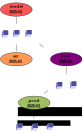
\includegraphics[width=0.4\columnwidth]{cylc-io}
  \caption{Example High-Level Workflow}
  \label{fig:cylc-io}
\end{figure}

The trick part when we consider only the Tasks and not the datasets in the workflow is that it may lead to the false impression that the Tasks only depend on the immediate previous one. For that, we have an example in Figure \ref{fig:cylc-io-model-3} showing that Task \texttt{prod} depends directly of Task \texttt{post} (Dataset I/O 4) and indirectly of Task \texttt{model} (Dataset I/O 2). Once all this dependencies are represented in the workflow, then the storage for all datasets can be optimised.

\begin{figure}[H]
  \centering
  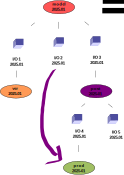
\includegraphics[width=0.6\columnwidth]{cylc-io-model-3}
  \caption{First Stage Workflow}
  \label{fig:cylc-io-model-3}
\end{figure}

The focus of this paper is to exemplify the I/O optimisations that can be made if the datasets dependencies are established. This information in fact is presented in the workflows prior to the Cylc application, so nothing else will be required from the user. But to have the information explicitly, Cylc need some changes to be able to:

\begin{enumerate}

\item deliver it together with the workflow, and

\item adapt the resulting workflow to consider the I/O modifications.

\end{enumerate}

The information about the system architecture can be provided in advance. If that is not possible, we can use monitoring to identify both the architecture and the I/O patterns for the workflow. For that, all we need is to run one cycle of the workflow and detect the patterns associated with it. For this purpose, we intend to use Machine Learning to identify the patterns and adapt the workflow in case of unexpected situations (system is down, nodes are unresponsive, etc.).

With this separation of concepts, we can abstract from the worflow what is essential and has to be provided by the user and what a machine should optimise to ensure that the resources available are being used smartly. Everytime parameters are manually tuned, that has a room from improvement by using automatised decision making. And Machine Learning is proven effective in replacing human-beings in several problems.

About the I/O, the optimisations we can envision are related to the life cycle of datasets and the placement of such datasets into specific memory according to their utilisation. What happens in most current workflows is that usually they use only two types of file systems: \textbf{work} and \textbf{local}. When a task is set to computing, the corresponding dataset is moved to local, processed, and the resulting datasets are moved back to \textbf{work}. If the local filesystem achieves its capacity, then the datasets move back to \textbf{work} and keep running the task until is finished. If the I/O planning is made a priori, this situation can be avoided.

\begin{description}

\item{NFS} Relatively slow, persistent file system - Nightly incremental backups

\item{Lustre} Large, fast distributed scratch file system - No backups

\url{https://info.hpc.sussex.ac.uk/hpc-guide/storage.html}

\end{description}

In addition to the fyle systems described, many supercomputers have also available for the user \textbf{scratch} fyle systems (sometimes local and global). So, in a real scenario, if the architecture of the machine is known, we can better use its resources.

\begin{figure}[H]
  \centering
  \includegraphics[width=0.6\columnwidth]{move}
  \caption{Some figure like this one indicating the movements among file systems. There are a lot of them in D4.2.}
  \label{fig:move}
\end{figure}


\end{document}
